\chapter{Background}
\label{chapter:background}
\thispagestyle{myheadings}

\graphicspath{{1a_background/Figures/}}

This work was motivated by the desire to scale microfluidic devices using automation techniques derived from the evolution of microelectronics. The emergence of microfluidic large scale integration (mLSI) resulted in the formulation of methods to manage complexity in design and fabrication. These methods often draw analogies with design and computation using microelectronics \cite{minhass2013}. Unfortunately, these efforts can often be disjointed --- automated design methods rely on manually-intensive fabrication efforts, or vice versa. What results from a unification of these efforts is a design-to-device workflow made possible by a new microfluidic fabrication framework that better utilizes automation via computer-aided manufacturing (CAM) at a lower cost in both time and money when compared to the traditional fabrication framework, namely soft lithography, which is outlined in Section 

This section provides a brief overview of the microfluidic--microelectronic analogy and highlights areas of deviation that may be inhibiting the microfluidic discipline from achieving the ubiquitousness and ease of use inherent to mLSI's \emph{in silico} counterpart: low-cost, rapid manufacturing and programmability.

%\section{The Microfluidic--Microelectronic Analogy}
%\label{sec:backgroundMF}
%It is difficult to imagine a computer engineer having to create a VLSI layout and fabricate an ASIC every time they wanted to run a C program. While there will always be a place for custom circuit design in the world of digital electronics one basic tenant of digital design, namely abstraction, requires that it remain very much the exception rather than the rule. Unfortunately for the experimentalist, this is not the case in the field of microfluidics. The creation of custom, ``one-off'', designs for individual microfluidic experiments, no matter how user-friendly the corresponding CAD software is, could be is what is keeping the productivity of mLSI chips from achieving that of its silicon counterparts. Since Thorsen \emph{et al.} successfully integrated thousands of micromechanical valves in 2002 \cite{thorsen2002}, academic researchers have attempted to manage exponentially greater complexity in microfluidic design via the introduction of new design methodologies that attempt to introduce ``top-down'' specificity and move away from a ``bottom-up'' design philosophy \cite{minhass2013}\cite{melin2007}\cite{minhass2012} yet microfluidic experimentalists still find themselves in front of an oven baking a photoresist until it ceases to be sticky. 

%Managing complexity is a necessary craft in that it allows the engineer to design complicated systems without becoming overwhelmed by details. The art of managing complexity in digital electronics design is  a mature process relative to that found in microfluidics. This is evident by the existence of larger scales of integration \emph{in silico}, such as VLSI, and by microfluidic efforts to create tools that mirror the design-to-execution workflow found in electronic computing. Examples of such tools are Micado, for automation of control layer routing \cite{amin2009}, and BioStream \cite{thies2008}, which could serve as the cornerstone of true experimental automation and will be described in the subsequent section. It could serve as a useful exercise to emphasize one methodology used to design and fabricate microelectronics while managing complexity and then contrast this principle with the current state of microfluidic design. There are few better places to find fundamental digital design practices than in introductory textbooks, one of which lists abstraction as the most important element of managing complexity \cite{Harris+Harris}.

If the goal is true experimental automation, then the expensive and time-consuming fabrication step should be removed from the work flow for the majority case as it is for electronic computation. Often, academic papers delving into the relm of mLSI begin by presenting an analogy between microfluidic LSI and LSI found in digital electronics. This research analogy seems strange as computer engineers can be productive using programmable tools (e.g., personal computers, Field Programmable Gate Arrays (FPGA), etc.) without having to know how to wash chemical from printed circuit boards (PCBs), use CAD tools to layout application specific integrated circuits (ASICs), or enlist the aid of experts in fabrication who can. Thus, the \emph{in silico} analogy does not hold when applied to the common-use case: that of the individual scientist or engineer.

Chapter \ref{chapter:xposer} outlines a novel primitive for continuous-flow microfluidics aimed at unlocking elements of programmability in continuous-flow devices. It analyzes and solves microfluidic design challenges using tools for automated design and control, ultimately providing a solution that would allow the microfluidic experimentalist to be one step closer to realizing the productivity potential of true large-scale integration. 

\subsection{Microfluidic Design Tools}
\label{ssec:DesignTools}

Abstraction works by placing the user at only the highest level relevant to the computation being performed and masking all underlying details. It can, therefore, be contended that functionally complete automation of microfluidic experiments implies placing the scientist at only the highest levels of abstraction and masking all underlying details. Currently, even the best efforts in microfluidic tools only remove intermediate levels of abstraction, while exposing the scientist to the highest \textbf{and lowest} levels. Imagine if the only output of a C program were a circuit schematic that must first be built in order to obtain the result of the program. The use of the term ``working levels'' of complexity implies that the person operating within that layer need not concern themselves with the details of a lower layer, as such requirements would ultimately defeat the purpose of abstraction. Lower levels of detail are said to be ``abstracted'' away when their use is considered automatic. However, designers of systems residing in one particular abstraction layer should have an understanding of how their design decisions affect the layers immediately above and below the working layer, such as a C programmer understanding the nature of an address space \cite{Harris+Harris}. Theis \emph{et al} advocate for the creation of abstraction layers in microfluidics similar to that found in electronic computing \cite{thies2008}. These layers achieve success by focusing on three basic fluidic operations: mixing, transport and storage. Their BioStream protocol is a good first step in decoupling microfluidic architecture from biological computation by providing a common language for describing an experimental protocol. BioStream served initially as a standard language for reporting biological protocols but expanded to an end-to-end system that effectively describes biological protocols within the BioStream Fluidic ISA and executes them at the hardware level independent of microfluidic chip microarchitecture \cite{thies2008}. BioStream, however, does not fully address a functional purpose of abstraction, which is to provide automation, but it does accomplish a very important step the authors describe as a ``division of labor'' between the biology and microfluidic experts. 
There is, and probably always will be, a place in digital electronics for PCB design and ASIC fabrication. However, before an engineer decides to begin the process of building a custom PCB or layout a new ASIC they should first consider how their deisgn decision addresses the productivity gap. In order to proceed, a working definition of the term ``productivity'' must be presented. Process and requirements engineers \cite{Review_ProcessEngr} have defined productivity strictly in terms of hours saved \cite{CostBenefit_hours}, as a function of on-time delivery \cite{OnTimeDelivery} or as some measure of quality \cite{Quality}. This paper will define the productivity of a particular method as the number of hours saved through the implementation of a particular process.

Device fabrication is not a task oft performed by a computer scientist. Rather, a computer scientist spends many hours debugging a program such that it runs reliably and correctly within the confines of a particular ISA. This exemplifies the nature of design discipline. It is well-within the realm of possibility for a computer engineer to give up debugging a program and reach for a CAD tool, with which to build a custom chip designed for their particular purposes. That scenario would only make sense if the final custom-fabricated solution could overcome the extremely large gap in productivity inherent to designing and fabricating it. The amount of lead-time required to design and build an ASIC or PCB could significantly outweigh the benefits of having a single custom-chip to use only in very specific circumstances and only within that one engineer's lab. Why then is this practice deemed acceptable in microfluidics?

Even attempts to create some framework for flow-based microfluidic design, such as a common microfluidic ISA\cite{amin2009} or predefined software modules \cite{soe2013} are still, fundamentally, design methods for chip fabrication. Microfluidic chip fabrication is a highly unproductive in that it requires many hours to design and build a device incapable of performing diverse and repeatable experiments. Fortunately for the computer engineer there exists other prototyping options besides PCBs and ASICs, such as the use of a field programmable gate array (FPGA) or microcontroller. The microfluidic experimentalist is left with only one prototyping option that almost always requires some level of device
fabrication.


\subsection{Microfluidic Fabrication Using Soft Lithography}
\label{ssec:backgroundSL}

\textbf{EDIT THIS: IT'S FROM CASSIE'S THESIS}
Soft lithography was adopted as the traditional method of fabricating microfluidics based on the success photolithography demonstrated in fabricating microelectronics \cite{whitesides2006}. microfluidics based on the Microfluidic chips are fabricated from PDMS through soft lithography. As many detailed reviews of the process exist \cite{duffy1998}\cite{sia2003}\cite{weibel2007}, I will only provide a brief description. Photoresist (typically SU-8) is spun out over a substrate of silicon, and a transparency with the chip design is placed over it as a mask. The sandwich of mask, photoresist, and substrate is then exposed to UV light. The mask is removed, and the photoresist washed in developing agent to obtain the master mold. PDMS layers are cast from the master through replica molding. The channels are then sealed against a substrate suitable for imaging and connected to input and control structures. A summary of the process is shown in Figure 2·2A. The entire fabrication process, from the creation of the photomask to the molding of the chip, takes no more than a few days including the turnaround time for printing the photomask. This process does require the experimenter to have access to a high quality cleanroom and purchase specialized fabrication equipment for soft lithography (Elveflow, 2015), or else contract out the fabrication process to a dedicated microfluidic foundry.
\textbf{STOP}

\begin{figure}[h]
  \begin{minipage}[t]{0.75\linewidth}\centering
    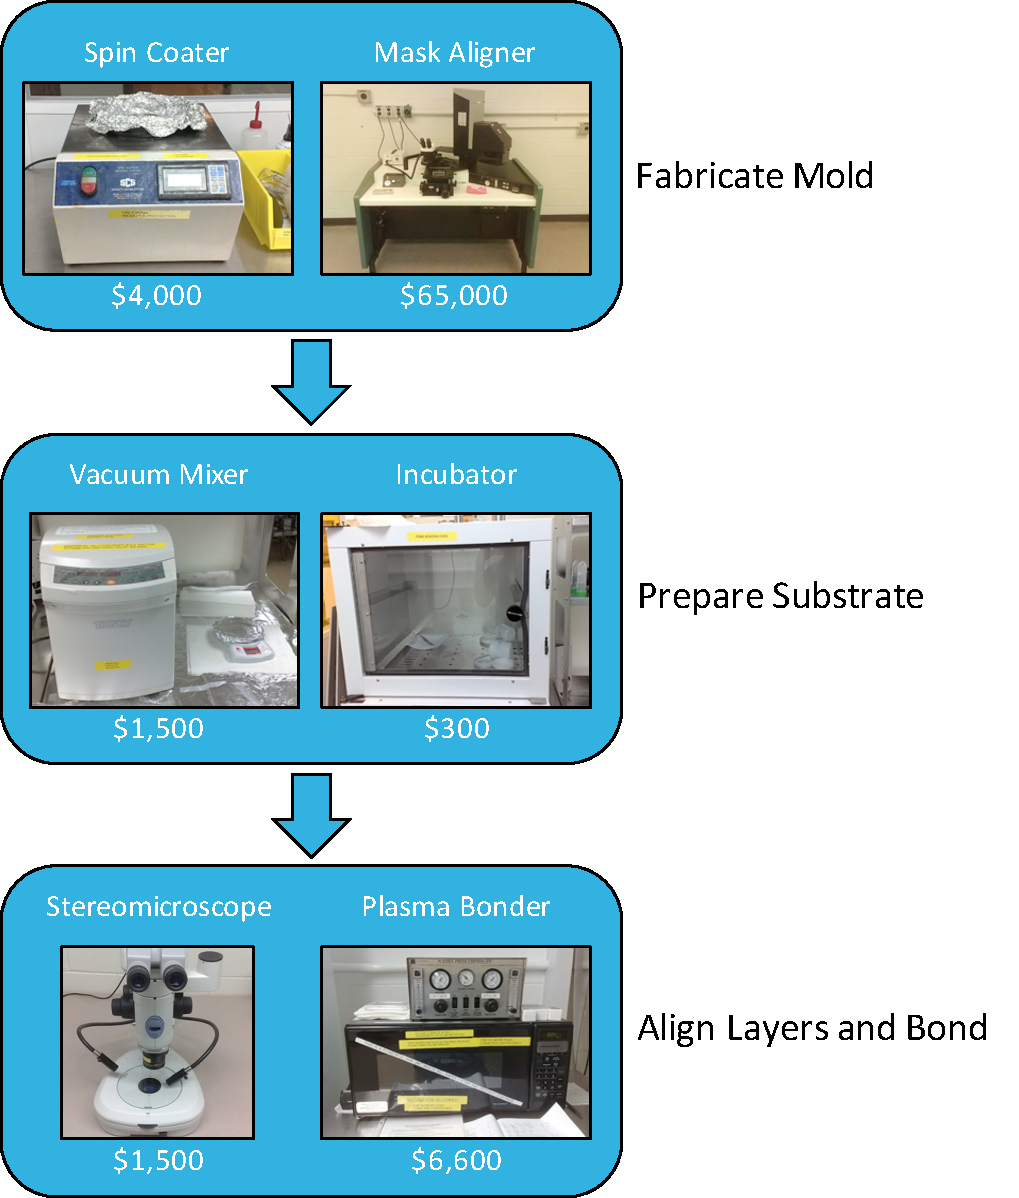
\includegraphics[width=14cm]{equipSoftLith.pdf}
    \medskip
  \end{minipage}\hfill
  \caption[Specialized equipment required to performform soft lithography]{Microfluidic fabrication via multi-layer soft lithography requires about \$80,000 in specialized equipment, not accounting for infrastructure, personnel, maintenance, or training. Cost estimates based on company quotes.}
    \label{fig:equipSoftLith}
\end{figure}


\section{Continuous-Flow Microfluidic Routing}
\label{sec:backgroundCFRouting}

It is difficult to imagine a computer engineer having to create a VLSI layout and fabricate an ASIC every time they wanted to run a C program. While there will always be a place for custom circuit design in the world of digital electronics, the basic tenants of digital design require that it remain very much the exception rather than the rule. Unfortunately for the experimentalist, this is not the case in the field of microfluidics. The creation of custom, ``one-off'', designs for individual microfluidic experiments, no matter how user-friendly the corresponding CAD software is, could be is what is keeping the productivity of mLSI chips from achieving that of its silicon counterparts. Since Thorsen \emph{et al.} successfully integrated thousands of micromechanical valves in 2002 \cite{thorsen2002}, academic researchers have attempted to manage exponentially greater complexity in microfluidic design via the introduction of new design methodologies that attempt to introduce ``top-down'' specificity and move away from a ``bottom-up'' design philosophy \cite{minhass2013}\cite{melin2007}\cite{minhass2012} yet microfluidic experimentalists still find themselves in front of an oven baking a photoresist until it ceases to be sticky. If the goal is true experimental automation, then the expensive and time-consuming fabrication step must be removed from the work flow for the majority case as it is for electronic computation. Often, academic papers delving into the relm of mLSI begin by presenting an analogy between microfluidic LSI and LSI found in digital electronics. This analogy seems strange as computer engineers can be productive without having to know how to wash chemical from printed circuit boards (PCBs), use CAD tools to layout application specific integrated circuits (ASICs), or enlist the aid of experts in fabrication who can. Thus, the \emph{in silico} analogy does not hold when applied to the common-use case: that of the individual scientist or engineer. Why is that? This paper will provide a possible answer via a historical analysis of the emergence of digital electronics design and highlight instances where microfluidics deviated, resulting in the current design topology seen today. It will also analyze various attempts to rectify microfluidic design challenges using various computer-aided tools and possibly provide the missing element that would allow the microfluidic experimentalist to be one step closer to realizing the productivity potential of true large-scale integration. 



\section{Acoustofluidic Cell Separation}
\label{sec:cellSep}
